\section{GPIO (General Purpose I/O)}

\subsection{GPIO Fundamentals}

\begin{definition}{GPIO}\\
    \textbf{Situation:}
    \begin{itemize}
        \item Microcontroller as a general purpose device
        \item Many functional blocks included
    \end{itemize}

    \textbf{Problem:}
    \begin{itemize}
        \item Limited number of pins
        \item Many functions to be implemented (many functional blocks included)
    \end{itemize}

    \textbf{Solution:}
    \begin{itemize}
        \item Many (all) pins are configurable as GPIO
        \item Select the needed I/O pins and functions
        \item \oq pin sharing\cq
        \item Output multiplexer needs to be configured
    \end{itemize}
\end{definition}

\begin{concept}{GPIO Overview}\\
General Purpose Input/Output (GPIO) pins allow the microcontroller to interact with the external world.
\begin{itemize}
    \item Pins can be configured as digital inputs or outputs
    \item Most pins support multiple functions (pin sharing) through internal multiplexers
    \item Configuration is done through memory-mapped registers
    \item Each GPIO port typically has 16 pins (e.g., GPIOA, GPIOB, etc.)
\end{itemize}
\end{concept}

\begin{definition}{Pin Sharing}\\
Multiple functions can share a single physical pin:
\begin{itemize}
    \item Digital inputs/outputs (GPIO)
    \item Serial interfaces (UART, SPI, I2C)
    \item Timers/Counters
    \item ADC (Analog-to-Digital Conversion)
    \item Alternate functions
\end{itemize}
Not all functions can be used simultaneously; configuration registers define pin usage.
\end{definition}

\subsection{GPIO Structure}

\begin{definition}{GPIO Registers}\\
Each GPIO port has several configuration registers:
\begin{itemize}
    \item \textbf{GPIOx\_MODER}: Mode register (input, output, alternate function, analog) - configures pin as input or output (direction control)
    \item \textbf{GPIOx\_OTYPER}: Output type register (push-pull or open-drain)
    \item \textbf{GPIOx\_OSPEEDR}: Output speed register (low, medium, high, very high) - configures speed
    \item \textbf{GPIOx\_PUPDR}: Pull-up/pull-down register
    \item \textbf{GPIOx\_IDR}: Input data register (read-only) - reads the pin state
    \item \textbf{GPIOx\_ODR}: Output data register (read/write) - sets the output state
    \item \textbf{GPIOx\_BSRR}: Bit set/reset register (atomic operations)
    \item \textbf{GPIOx\_LCKR}: Configuration lock register
    \item \textbf{GPIOx\_AFRL/H}: Alternate function registers (AF selection for pins 0-7 and 8-15)
\end{itemize}
\end{definition}

\begin{concept}{Structure}\\
    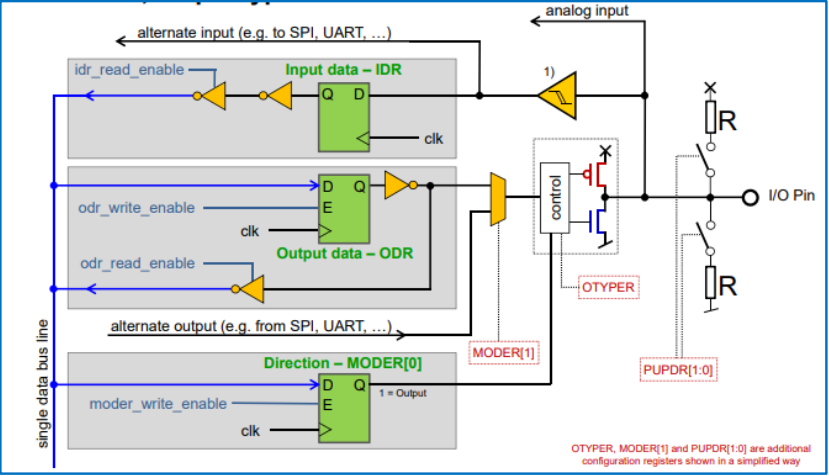
\includegraphics[width=\linewidth]{structure_gpio.png}
\end{concept}



\subsubsection{Push-Pull vs. Open-Drain}

\begin{concept}{Push-Pull vs Open-Drain Outputs}
\begin{itemize}
    \item \textbf{Push-Pull:}
    \begin{itemize}
        \item Can actively drive output high (to VDD) or low (to GND)
        \item Faster switching times, can source and sink current
        \item Default output mode for GPIO pins
    \end{itemize}
    \item \textbf{Open-Drain:}
    \begin{itemize}
        \item Can only actively drive output low
        \item Relies on external pull-up resistor to reach high state
        \item Multiple devices can share a line without conflicts (e.g., I2C bus)
        \item Used in "wired-AND" configurations
    \end{itemize}
\end{itemize}
\end{concept}

\subsubsection{GPIO Configuration}

\begin{definition}{Direction Configuration (MODER)}\\
The GPIOx\_MODER register configures each pin's direction:
\begin{itemize}
    \item \textbf{00}: Input mode
    \item \textbf{01}: General purpose output mode
    \item \textbf{10}: Alternate function mode
    \item \textbf{11}: Analog mode
\end{itemize}
Each pin uses 2 bits in the register, allowing for 16 pins per port.
\end{definition}

\begin{definition}{Output Type (OTYPER)}\\
The GPIOx\_OTYPER register configures the output driver type:
\begin{itemize}
    \item \textbf{0}: Push-pull (can actively drive high or low)
    \item \textbf{1}: Open-drain (can drive low, relies on external pull-up for high)
\end{itemize}
\end{definition}

\begin{definition}{Pull-up/Pull-down (PUPDR)}\\
The GPIOx\_PUPDR register configures internal resistors:
\begin{itemize}
    \item \textbf{00}: No pull-up, no pull-down
    \item \textbf{01}: Pull-up
    \item \textbf{10}: Pull-down
    \item \textbf{11}: Reserved
\end{itemize}
\end{definition}

\begin{definition}{Speed Configuration (OSPEEDR)}\\
The GPIOx\_OSPEEDR register configures the output slew rate:
\begin{itemize}
    \item \textbf{00}: Low speed
    \item \textbf{01}: Medium speed
    \item \textbf{10}: High speed
    \item \textbf{11}: Very high speed
\end{itemize}
\end{definition}

\begin{definition}{Input Data Register (IDR)}\\
The GPIOx\_IDR is a read-only register containing the input value of the corresponding I/O port.
\end{definition}

\begin{definition}{Output Data Register (ODR)}\\
The GPIOx\_ODR can be read and written to set the output state of GPIO pins.
\end{definition}

\begin{definition}{Bit Set/Reset Register (BSRR)}\\
The GPIOx\_BSRR allows atomic bit operations:
\begin{itemize}
    \item Bits [15:0]: Set corresponding ODR bit by writing '1'
    \item Bits [31:16]: Reset corresponding ODR bit by writing '1'
\end{itemize}
This ensures atomic access without read-modify-write operations.
\end{definition}

\begin{KR}{Setting and Clearing Bits} GPIOx\_BSRR
    \begin{itemize}
        \item 0-15: Set Bits $\rightarrow$ 1: Set, 0: No Change
        \item 16-31: Reset/Clear Bits $\rightarrow$ 1: Reset, 0: No Change
        \item Ensures atomic access in software (no interruption possible)
    \end{itemize}
\end{KR}

\begin{KR}{Configuring a GPIO Pin}
\paragraph{Step 1: Enable GPIO clock}
Enable the clock to the GPIO port using RCC register.
\paragraph{Step 2: Configure pin direction}
Set the mode register (MODER) to configure as input, output, etc.
\paragraph{Step 3: Configure additional properties}
Configure output type, speed, and pull-up/down as needed.
\paragraph{Step 4: Set initial state (for outputs)}
For output pins, set the initial state in ODR or using BSRR.

\begin{lstlisting}[language=C, style=basesmol] 
// Step 1: Enable GPIOA clock
RCC->AHB1ENR |= (1 << 0);  // Set bit 0 for GPIOA

// Step 2: Configure PA5 as output (bits 10-11 = 01)
GPIOA->MODER &= ~(3 << 10);  // Clear bits 10-11
GPIOA->MODER |= (1 << 10);   // Set as output

// Step 3: Configure as push-pull, high speed, no pull-up/down
GPIOA->OTYPER &= ~(1 << 5);     // Push-pull (clear bit 5)
GPIOA->OSPEEDR |= (3 << 10);    // Very high speed (set bits 10-11)
GPIOA->PUPDR &= ~(3 << 10);     // No pull-up/down (clear bits 10-11)

// Step 4: Set initial state (turn on LED)
GPIOA->ODR |= (1 << 5);         // Set PA5 high
// OR: Atomic set
GPIOA->BSRR = (1 << 5);         // Set PA5 high
\end{lstlisting}
\end{KR}

\begin{example2}{GPIO Configuration Exercise}\\
Configure pin PA3 as an output with open-drain configuration, low speed, and pull-up enabled. Then set the pin to low state.
\begin{lstlisting}[language=C, style=basesmol] 
// Enable GPIOA clock
RCC->AHB1ENR |= (1 << 0);  // Bit 0 for GPIOA

// Configure PA3 as output (bits 6-7 = 01)
GPIOA->MODER \&= ~(3 << 6);  // Clear bits 6-7
GPIOA->MODER |= (1 << 6);   // Set bit 6 (output mode)

// Configure as open-drain (bit 3 = 1)
GPIOA->OTYPER |= (1 << 3);  

// Configure as low speed (bits 6-7 = 00)
GPIOA->OSPEEDR \&= ~(3 << 6);  // Clear bits 6-7 (low speed)

// Configure with pull-up (bits 6-7 = 01)
GPIOA->PUPDR \&= ~(3 << 6);    // Clear bits 6-7
GPIOA->PUPDR |= (1 << 6);     // Set bit 6 (pull-up)

// Set pin to low state using BSRR
GPIOA->BSRR = (1 << (3 + 16));  // Set bit 19 (reset PA3)
\end{lstlisting}
\end{example2}

\subsection{Data Registers and Operations}

\subsubsection{Register Access}

\begin{formula}{Register Address} = Base address + Offset
    \begin{itemize}
        \item Offset is given for each register in reference Manual
        \item Base address is defined in memory map (reference manual)
    \end{itemize}
\end{formula}

\begin{corollary}{Data Operations}
    \begin{itemize}
        \item Input: Read register \textbf{GPIOx\_IDR} (Input Data Register)
        \item Output: Write register \textbf{GPIOx\_ODR} (Output Data Register) or \textbf{GPIOx\_BSRR} (Bit Set Reset Register)
    \end{itemize}
\end{corollary}




\begin{KR}{Reading and Writing GPIO}
\paragraph{Reading Input Pins}
Read the current state of GPIO pins using the IDR register.
\paragraph{Writing Output Pins - Using ODR}
Set or clear output pins by modifying the ODR register.
\paragraph{Writing Output Pins - Using BSRR (preferred)}
Set or clear output pins atomically using the BSRR register.

\begin{lstlisting}[language=C, style=basesmol] 
// Reading input from GPIOA pin 0
uint32_t buttonState = (GPIOA->IDR & (1 << 0)) != 0;

// Writing output using ODR (not atomic)
// Set pin high
GPIOA->ODR |= (1 << 5);
// Set pin low
GPIOA->ODR &= ~(1 << 5);

// Writing output using BSRR (atomic)
// Set pin high (bits 0-15)
GPIOA->BSRR = (1 << 5);
// Set pin low (bits 16-31)
GPIOA->BSRR = (1 << (5 + 16));
\end{lstlisting}
\end{KR}



\subsection{Hardware Abstraction Layer (HAL)}

\begin{definition}{Hardware Abstraction Layer (HAL)}\\
    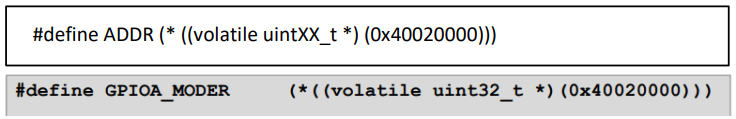
\includegraphics[width=\linewidth]{HAL1.png}\\
    \textbf{Accessing a register:}
    \begin{itemize}
        \item each GPIO port has the same 10 registers 
        \item there are 11 GPIO ports $\rightarrow$ GPIOA to GPIOI
    \end{itemize}
    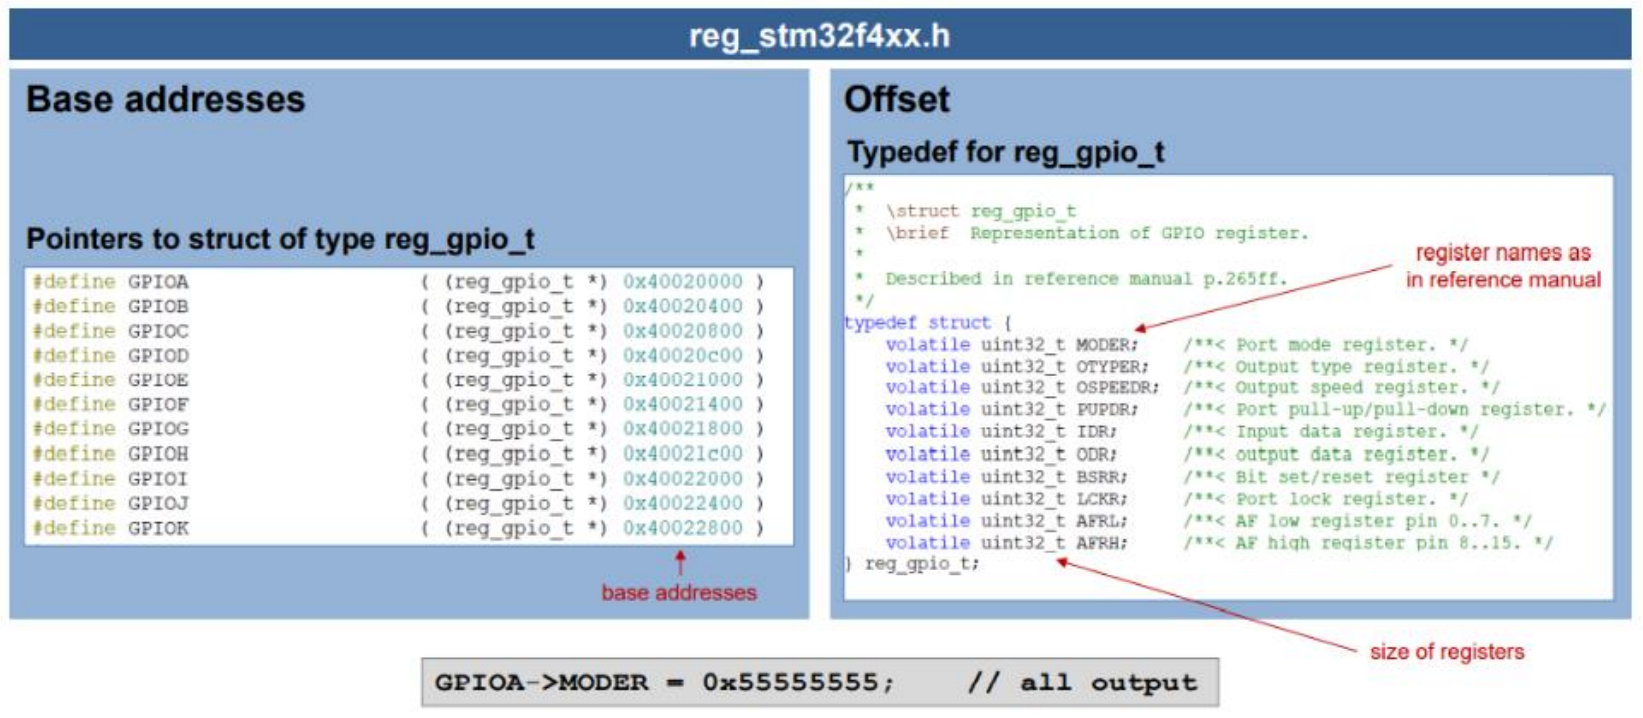
\includegraphics[width=\linewidth]{HAL2.png}
\end{definition}

\begin{concept}{HAL for GPIO}\\
The Hardware Abstraction Layer provides a structured way to access GPIO registers:
\begin{itemize}
    \item Based on structs that map to hardware registers
    \item Typedef for register structure (e.g., \texttt{reg\_gpio\_t})
    \item Pointers to each GPIO port (e.g., \texttt{GPIOA}, \texttt{GPIOB})
    \item Base addresses defined in header file
    \item Helper macros for bit manipulation
\end{itemize}
This approach makes code more readable and maintainable than direct register address manipulation.
\end{concept}

\begin{code}{Using HAL for GPIO}
\begin{lstlisting}[language=C, style=basesmol] 
// Using HAL style access
#include "reg_stm32f4xx.h"  // Contains structure definitions

// Configure PA3 as output
GPIOA->MODER &= ~(3 << 6);  // Clear bits 6-7
GPIOA->MODER |= (1 << 6);   // Set bit 6 (output mode)

// Instead of direct register access:
// volatile uint32_t *reg = (volatile uint32_t *)(0x40020000);
// *reg &= ~(3 << 6);
// *reg |= (1 << 6);
\end{lstlisting}
\end{code}


\section{GPIO}
\subsubsection{General Purpose Input Output}




\subsection{Conclusion}

\begin{KR}{Conclusion}
\end{KR}

\begin{remark}
    Learning Objectives:
    At the end of this lesson, you will be able
    - to work with register descriptions in reference manuals
    - to explain the concept and implementation of GPIOs
    - to explain the differences between open-drain and push-pull
    - to use GPIOs in your own programs
    - to explain the idea of a HAL
\end{remark}

\section{General Purpose I/O (GPIO) Exercises}

\subsection{GPIO Configuration and Programming}

\begin{KR}{Configuring GPIO Pins}\\
\paragraph{Identify GPIO port and pin}
\begin{itemize}
    \item Find the port letter (A-K) and pin number (0-15) from documentation
    \item Look up the corresponding pin number on the microcontroller package
\end{itemize}

\paragraph{Calculate register addresses}
\begin{itemize}
    \item Find the base address for the GPIO port in the memory map
    \item Calculate register addresses by adding offsets to the base address
    \item For STM32F4: Base addresses are at 0x4002 0000 + (0x400 * port\_index)
    \begin{itemize}
        \item GPIOA: 0x4002 0000
        \item GPIOB: 0x4002 0400
        \item GPIOC: 0x4002 0800
        \item And so on...
    \end{itemize}
\end{itemize}

\paragraph{Configure GPIO mode}
\begin{itemize}
    \item Use GPIOx\_MODER register to set pin mode:
    \begin{itemize}
        \item 00: Input mode
        \item 01: General purpose output mode
        \item 10: Alternate function mode
        \item 11: Analog mode
    \end{itemize}
    \item Each pin requires 2 bits, so pin n uses bits 2n+1:2n
\end{itemize}

\paragraph{Configure output type (for output mode)}
\begin{itemize}
    \item Use GPIOx\_OTYPER register:
    \begin{itemize}
        \item 0: Push-pull output (can drive high or low)
        \item 1: Open-drain output (can drive low only)
    \end{itemize}
\end{itemize}

\paragraph{Configure pull-up/pull-down resistors}
\begin{itemize}
    \item Use GPIOx\_PUPDR register:
    \begin{itemize}
        \item 00: No pull-up, no pull-down
        \item 01: Pull-up
        \item 10: Pull-down
        \item 11: Reserved
    \end{itemize}
    \item Each pin requires 2 bits, so pin n uses bits 2n+1:2n
\end{itemize}

\paragraph{Configure speed (for output mode)}
\begin{itemize}
    \item Use GPIOx\_OSPEEDR register:
    \begin{itemize}
        \item 00: Low speed
        \item 01: Medium speed
        \item 10: High speed
        \item 11: Very high speed
    \end{itemize}
    \item Each pin requires 2 bits, so pin n uses bits 2n+1:2n
\end{itemize}

\paragraph{Enable clock for GPIO port}
\begin{itemize}
    \item Use RCC\_AHB1ENR register to enable clock for the GPIO port
    \item Set the corresponding bit for the port
\end{itemize}
\end{KR}

\begin{example2}{GPIO Configuration Example}\\
Configure pin PA3 as a low-speed, open-drain output with pull-up.

\tcblower
\paragraph{Solution:}
First, identify the registers and their addresses:
\begin{itemize}
    \item GPIOA base address: 0x4002 0000
    \item GPIOA\_MODER: 0x4002 0000 (offset 0x00)
    \item GPIOA\_OTYPER: 0x4002 0004 (offset 0x04)
    \item GPIOA\_OSPEEDR: 0x4002 0008 (offset 0x08)
    \item GPIOA\_PUPDR: 0x4002 000C (offset 0x0C)
\end{itemize}

Then, calculate the bit fields for pin 3:
\begin{itemize}
    \item MODER3[1:0] = 01 (output mode) at bits 7:6
    \item OTYPER3 = 1 (open-drain) at bit 3
    \item OSPEEDR3[1:0] = 00 (low speed) at bits 7:6
    \item PUPDR3[1:0] = 01 (pull-up) at bits 7:6
\end{itemize}

C code to configure the pin:
\begin{lstlisting}[language=C, style=basesmol]
// Enable clock for GPIOA
RCC->AHB1ENR |= (1 << 0);

// Configure PA3 as output (01)
// Clear bits 7:6 then set bit 6
GPIOA->MODER &= ~(0x3 << 6);
GPIOA->MODER |= (0x1 << 6);

// Configure as open-drain (1)
GPIOA->OTYPER |= (1 << 3);

// Configure as low speed (00)
GPIOA->OSPEEDR &= ~(0x3 << 6);

// Configure with pull-up (01)
GPIOA->PUPDR &= ~(0x3 << 6);
GPIOA->PUPDR |= (0x1 << 6);
\end{lstlisting}
\end{example2}

\begin{KR}{Using GPIO Data Registers}\\
\paragraph{Reading input pins}
\begin{itemize}
    \item Use GPIOx\_IDR register to read the state of input pins
    \item Bit n corresponds to pin n (0-15)
    \item Apply appropriate bit mask to extract the bit(s) of interest
\end{itemize}

\paragraph{Writing output pins}
\begin{itemize}
    \item Use GPIOx\_ODR register to write to output pins
    \item Bit n corresponds to pin n (0-15)
    \item Writing to ODR affects all bits at once, which can lead to race conditions
\end{itemize}

\paragraph{Atomic bit manipulation}
\begin{itemize}
    \item Use GPIOx\_BSRR register for atomic bit setting/clearing:
    \begin{itemize}
        \item Bits 15:0: Setting corresponding ODR bits (write 1 to set)
        \item Bits 31:16: Clearing corresponding ODR bits (write 1 to clear)
    \end{itemize}
    \item Example: To set pin 5, write (1 << 5) to BSRR
    \item Example: To clear pin 5, write (1 << (16+5)) to BSRR
\end{itemize}
\end{KR}

\begin{example2}{GPIO Data Operations Example}\\
Write code to:
\begin{enumerate}
    \item Read the state of user button B1 on port A, pin 0
    \item Turn on the green LED LD3 on port G, pin 13 when B1 is pressed
    \item Turn on the red LED LD4 on port G, pin 14 when B1 is not pressed
\end{enumerate}

\tcblower
\paragraph{Solution:}
First, define the register addresses and pin mappings:

\begin{lstlisting}[language=C, style=basesmol]
// Button B1 is on PA0
// Green LED LD3 is on PG13
// Red LED LD4 is on PG14

#include "reg_stm32f4xx.h"

void button_led_control(void) {
    // Read button state (PA0)
    uint32_t button_state = GPIOA->IDR & (1 << 0);
    
    if (button_state) {
        // Button pressed - turn on green LED (PG13) and turn off red LED (PG14)
        // Set bit 13, clear bit 14 atomically
        GPIOG->BSRR = (1 << 13) | (1 << (16+14));
    } else {
        // Button not pressed - turn on red LED (PG14) and turn off green LED (PG13)
        // Set bit 14, clear bit 13 atomically
        GPIOG->BSRR = (1 << 14) | (1 << (16+13));
    }
}
\end{lstlisting}

Note: This assumes that the GPIO ports have been properly configured:
\begin{itemize}
    \item PA0 (Button B1) as input with pull-up/pull-down as needed
    \item PG13 (LED LD3) as push-pull output
    \item PG14 (LED LD4) as push-pull output
\end{itemize}
\end{example2}
